%=========================================================
% Clock and Reset for SoC
%=========================================================
\section{Clock \& Reset for SoC}
\label{sec:CLOCKRESETSOC}

The clock structure of the SoC is shown in Figure \ref{fig:CLOCKSOC}. For simulation, an internal clock clk01 is directly connected to the external clock input CLK50. For FPGA, the clk01 is generated by a PLL, and its frequency is 20MHz if the RV32F/RV32FC ISA are not implemented, or 16MHz if they are implemented. On the other hand, a slow clock clk2 with a frequency of 100KHz is also generated. The system clock clk is selected from either clk01 or clk2 by a glitch-less selector as shown in Figure \ref{fig:GLITCHLESSSELECTOR}. The selection signal is the GPIO2[7] input from an external pin. The reason why such a slow clock clk2 can be selected as the system clock is to verify that the any magnitude of the ratio between the system clock (clk) frequency and the JTAG/cJTAG clock (TCK/TCKC) frequency is acceptable in the mmRISC-1 core.

\begin{figure}[H]
    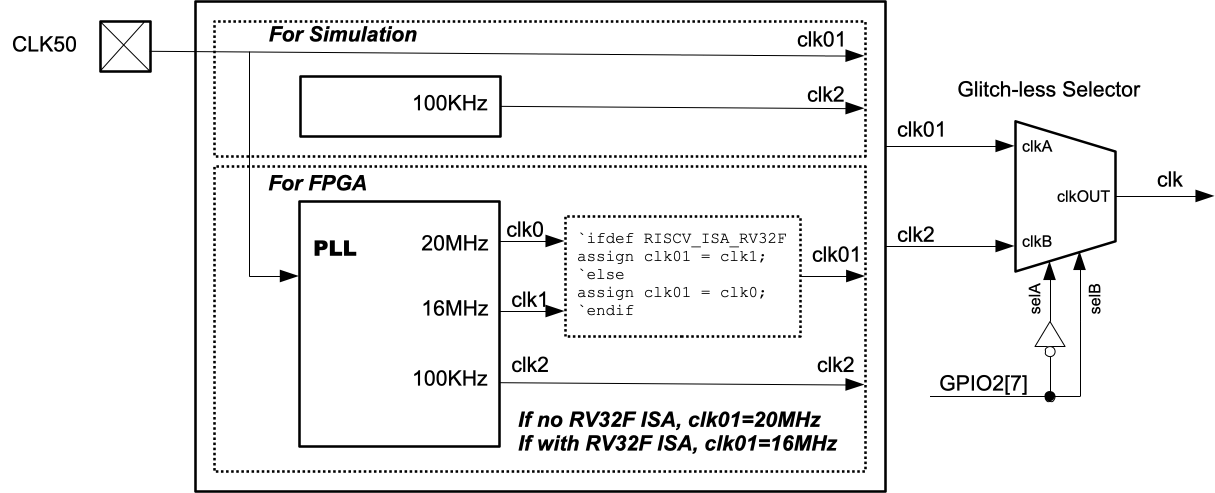
\includegraphics[width=1.00\columnwidth]{./Figure/ClockSoC.png}
    \caption{Clock Structure in Tiny SoC}
    \label{fig:CLOCKSOC}
\end{figure}

\begin{figure}[H]
    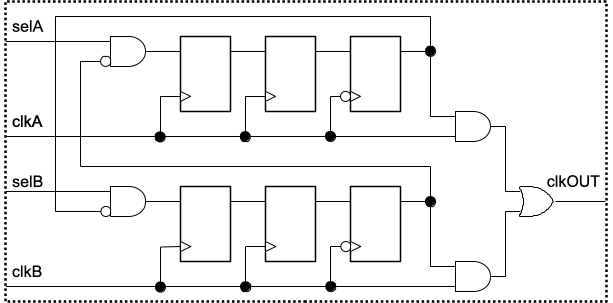
\includegraphics[width=0.6\columnwidth]{./Figure/GlitchlessSelector.png}
    \caption{Glitch-less Clock Selector}
    \label{fig:GLITCHLESSSELECTOR}
\end{figure}

Reset structure in the SoC is shown in Figure \ref{fig:RESETSOC}. Power on reset circuit is created using counter logic which is initialized at startup by an initial statement for simulation or by setting power-up-level parameters for FPGA. The power on reset signal and external reset input RES\_N are used as the source of RES\_ORG of mmRISC block. For FPGA, SRSTn\_IN of mmRISC block is simply from external reset input RES\_N and SRSTn\_OUT is not used. For simulation, SRSTn\_IN is from SRSTn and the SRSTn is driven by SRSTn\_OUT of mmRISC block. RES\_SYS output from mmRISC block is used as the reset of peripheral blocks. Reset structure in mmRISC block is shown in Figure \ref{fig:RESET}.

\begin{figure}[H]
    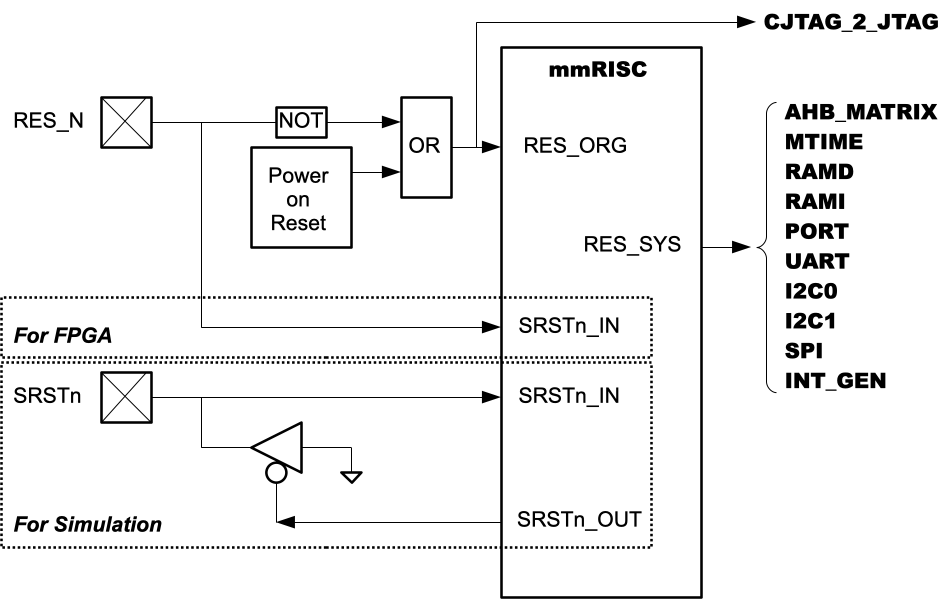
\includegraphics[width=1.00\columnwidth]{./Figure/ResetSoC.png}
    \caption{Reset Structure in Tiny SoC}
    \label{fig:RESETSOC}
\end{figure}

